\chapter{Management Summary}


\textbf{Context}

A big challenge of writing software has always been to keep the created source code manageable and maintainable. Early in the history of software development, modules have been used structure the code in manageable pieces and make it reusable. With the rise of networks and distributes systems, remote interfaces became popular and engineers started to implement services offering a remote interface to other components.

Several methodologies exist to guide a software architect when he designs services. \enquote{Service Oriented Architecture} is especially common in enterprise environments, the style of building microservices became popular in recent years. Leaving technical differences aside, both approaches share a common challenge: How can a big collection of data and functionality be decomposed into smaller pieces while retaining high cohesion and low coupling.

\textbf{A Structured Approach to Decoupling}

\begin{figure}
	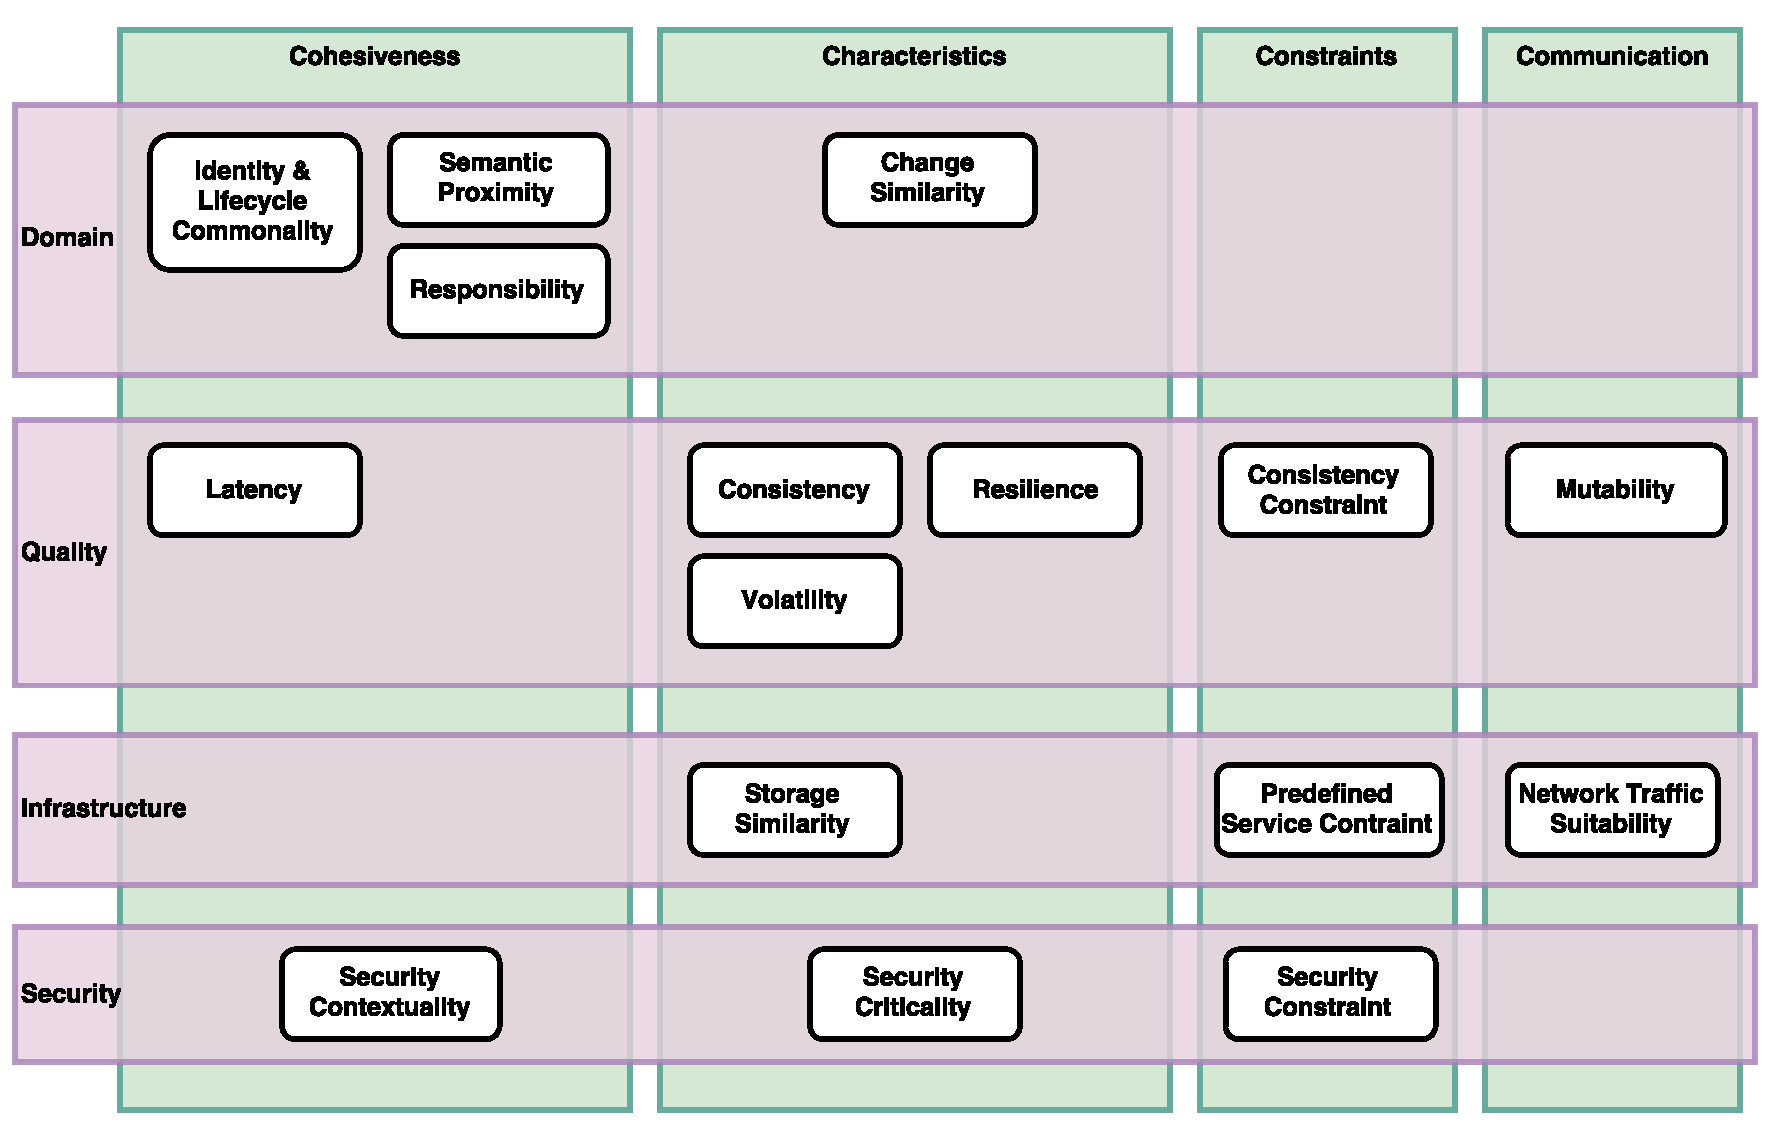
\includegraphics[scale=0.4]{diagrams/CouplingCatalog.pdf}
	\caption{Coupling criteria catalog}
	\label{fig:cc-catalog-mgmt-summary}
\end{figure}

When talking about cohesion and coupling we found that there is no extensive description in existing literature defining the actual factors thereof in distributed software systems. We therefore compiled a catalog of 14 coupling criteria that aims to form a comprehensive but not conclusive collection. 

Those coupling criteria help a software architect to structure internal and external dependencies. 

%TODO sollen wir die einzelnen kriterien hier auflisten?

Complementary to the coupling we also described an approach to quantify the coupling in a software system. We set nanoentities in relation to each other and assign a score to each tuple where a coupling exists. A score is a number between -10 and 10 given for a specific coupling criteria representing the strength of the coupling.

The exact importance of coupling is highly dependent on the context of a software system. Security and consistency for example are significantly divergent in a banking environment compared to an online social network. To reflect this we rate the coupling criteria using priorities before we sum it up to a final score.

All scores of coupling between nanoentities are collected and utilized to construct a weighted undirected graph. The vertices represent the nanoentities and the weighted edges embody the strength of the coupling between two nanoentities.

We implemented a tool called the \enquote{Service Cutter} as of a proof of concept of the scoring and decomposition approach.

\textbf{Suggested Service Cuts}

Once the graph is constructed, a graph clustering algorithm is used to calculate clusters so that as few edges as possible are cut. A cut edge equals with the coupling between the created services. This process produces candidate service cuts with high cohesion and low coupling.

We utilized two different algorithms to calculate the clusters. Girvan-Newman is deterministic and requires the desired number of clusters to be specified. The \enquote{Epidemic Label Propagation} algorithm by Raghavan and Leung is non-deterministic and computes the optimal number of clusters by itself. The two algorithms seem to be complementary and provide reasonable candidate service cuts. 

%TODO Screenshot Service Cutter

\textbf{Discussion}

We performed tests based on a imaginary \enquote{Trading System}, heavily inspired by real banking software, and the DDD sample application \enquote{Cargo Tracking}. On both domain models the Service Cutter suggests meaningful service cuts.

The topic of coupling in distributed systems is very broad and leaves a lot of room for further research. Out thesis suggests that coupling in software systems is quantifiable beyond the source code level.

\textbf{Outlook}

The current Service Cutter implementation is a proof of concept based on the already comprehensive coupling criteria catalog. Further projects should be focused on the many potential features described in the Future Work Chapter as well as further improvements of the scoring process and algorithms. The Service Cutter leaves room for enhancements on both side of the tool chain: Capturing data as well as providing reusable outputs.
